%\documentclass{beamer} 
\documentclass[handout]{beamer} % sin pausas
\usetheme{CambridgeUS}
%\setbeamertemplate{background}[grid][step=8 ] % cuadriculado


\usepackage{etex}
\usepackage{t1enc}
\usepackage[spanish,es-nodecimaldot]{babel}
\usepackage{latexsym}
\usepackage[utf8]{inputenc}
\usepackage{verbatim}
\usepackage{multicol}
\usepackage{amsgen,amsmath,amstext,amsbsy,amsopn,amsfonts,amssymb}
\usepackage{amsthm}
\usepackage{calc}         % From LaTeX distribution
\usepackage{graphicx}     % From LaTeX distribution
\usepackage{ifthen}
%\usepackage{makeidx}
\input{random.tex}        % From CTAN/macros/generic
\usepackage{subfigure} 
\usepackage{tikz}
\usepackage[customcolors]{hf-tikz}
\usetikzlibrary{arrows}
\usetikzlibrary{matrix}
\tikzset{
    every picture/.append style={
        execute at begin picture={\deactivatequoting},
        execute at end picture={\activatequoting}
    }
}
\usetikzlibrary{decorations.pathreplacing,angles,quotes}
\usetikzlibrary{shapes.geometric}
\usepackage{mathtools}
\usepackage{stackrel}
%\usepackage{enumerate}
\usepackage{enumitem}
\usepackage{tkz-graph}
\usepackage{polynom}
\polyset{%
    style=B,
    delims={(}{)},
    div=:
}
\renewcommand\labelitemi{$\circ$}
\setlist[enumerate]{label={(\arabic*)}}
\setbeamertemplate{itemize item}{$\circ$}
\setbeamertemplate{enumerate items}[default]
\definecolor{links}{HTML}{2A1B81}
\hypersetup{colorlinks,linkcolor=,urlcolor=links}


\newcommand{\Id}{\operatorname{Id}}
\newcommand{\img}{\operatorname{Im}}
\newcommand{\nuc}{\operatorname{Nu}}
\newcommand{\im}{\operatorname{Im}}
\renewcommand\nu{\operatorname{Nu}}
\newcommand{\la}{\langle}
\newcommand{\ra}{\rangle}
\renewcommand{\t}{{\operatorname{t}}}
\renewcommand{\sin}{{\,\operatorname{sen}}}
\newcommand{\Q}{\mathbb Q}
\newcommand{\R}{\mathbb R}
\newcommand{\C}{\mathbb C}
\newcommand{\K}{\mathbb K}
\newcommand{\F}{\mathbb F}
\newcommand{\Z}{\mathbb Z}
\newcommand{\N}{\mathbb N}
\newcommand\sgn{\operatorname{sgn}}
\renewcommand{\t}{{\operatorname{t}}}
\renewcommand{\figurename }{Figura}

%
% Ver http://joshua.smcvt.edu/latex2e/_005cnewenvironment-_0026-_005crenewenvironment.html
%

\renewenvironment{block}[1]% environment name
{% begin code
	\par\vskip .2cm%
	{\color{blue}#1}%
	\vskip .2cm
}%
{%
	\vskip .2cm}% end code


\renewenvironment{alertblock}[1]% environment name
{% begin code
	\par\vskip .2cm%
	{\color{red!80!black}#1}%
	\vskip .2cm
}%
{%
	\vskip .2cm}% end code


\renewenvironment{exampleblock}[1]% environment name
{% begin code
	\par\vskip .2cm%
	{\color{blue}#1}%
	\vskip .2cm
}%
{%
	\vskip .2cm}% end code




\newenvironment{exercise}[1]% environment name
{% begin code
	\par\vspace{\baselineskip}\noindent
	\textbf{Ejercicio (#1)}\begin{itshape}%
		\par\vspace{\baselineskip}\noindent\ignorespaces
	}%
	{% end code
	\end{itshape}\ignorespacesafterend
}


\newenvironment{definicion}[1][]% environment name
{% begin code
	\par\vskip .2cm%
	{\color{blue}Definición #1}%
	\vskip .2cm
}%
{%
	\vskip .2cm}% end code

    \newenvironment{notacion}[1][]% environment name
    {% begin code
        \par\vskip .2cm%
        {\color{blue}Notación #1}%
        \vskip .2cm
    }%
    {%
        \vskip .2cm}% end code

\newenvironment{observacion}[1][]% environment name
{% begin code
	\par\vskip .2cm%
	{\color{blue}Observación #1}%
	\vskip .2cm
}%
{%
	\vskip .2cm}% end code

\newenvironment{ejemplo}[1][]% environment name
{% begin code
	\par\vskip .2cm%
	{\color{blue}Ejemplo #1}%
	\vskip .2cm
}%
{%
	\vskip .2cm}% end code


\newenvironment{preguntas}[1][]% environment name
{% begin code
    \par\vskip .2cm%
    {\color{blue}Preguntas #1}%
    \vskip .2cm
}%
{%
    \vskip .2cm}% end code

\newenvironment{ejercicio}[1][]% environment name
{% begin code
	\par\vskip .2cm%
	{\color{blue}Ejercicio #1}%
	\vskip .2cm
}%
{%
	\vskip .2cm}% end code


\renewenvironment{proof}% environment name
{% begin code
	\par\vskip .2cm%
	{\color{blue}Demostración}%
	\vskip .2cm
}%
{%
	\vskip .2cm}% end code



\newenvironment{demostracion}% environment name
{% begin code
	\par\vskip .2cm%
	{\color{blue}Demostración}%
	\vskip .2cm
}%
{%
	\vskip .2cm}% end code

\newenvironment{idea}% environment name
{% begin code
	\par\vskip .2cm%
	{\color{blue}Idea de la demostración}%
	\vskip .2cm
}%
{%
	\vskip .2cm}% end code

\newenvironment{solucion}% environment name
{% begin code
	\par\vskip .2cm%
	{\color{blue}Solución}%
	\vskip .2cm
}%
{%
	\vskip .2cm}% end code



\newenvironment{lema}[1][]% environment name
{% begin code
	\par\vskip .2cm%
	{\color{blue}Lema #1}\begin{itshape}%
		\par\vskip .2cm
	}%
	{% end code
	\end{itshape}\vskip .2cm\ignorespacesafterend
}

\newenvironment{proposicion}[1][]% environment name
{% begin code
	\par\vskip .2cm%
	{\color{blue}Proposición #1}\begin{itshape}%
		\par\vskip .2cm
	}%
	{% end code
	\end{itshape}\vskip .2cm\ignorespacesafterend
}

\newenvironment{teorema}[1][]% environment name
{% begin code
	\par\vskip .2cm%
	{\color{blue}Teorema #1}\begin{itshape}%
		\par\vskip .2cm
	}%
	{% end code
	\end{itshape}\vskip .2cm\ignorespacesafterend
}


\newenvironment{corolario}[1][]% environment name
{% begin code
	\par\vskip .2cm%
	{\color{blue}Corolario #1}\begin{itshape}%
		\par\vskip .2cm
	}%
	{% end code
	\end{itshape}\vskip .2cm\ignorespacesafterend
}

\newenvironment{propiedad}% environment name
{% begin code
	\par\vskip .2cm%
	{\color{blue}Propiedad}\begin{itshape}%
		\par\vskip .2cm
	}%
	{% end code
	\end{itshape}\vskip .2cm\ignorespacesafterend
}

\newenvironment{conclusion}% environment name
{% begin code
	\par\vskip .2cm%
	{\color{blue}Conclusión}\begin{itshape}%
		\par\vskip .2cm
	}%
	{% end code
	\end{itshape}\vskip .2cm\ignorespacesafterend
}


\newenvironment{definicion*}% environment name
{% begin code
	\par\vskip .2cm%
	{\color{blue}Definición}%
	\vskip .2cm
}%
{%
	\vskip .2cm}% end code

\newenvironment{observacion*}% environment name
{% begin code
	\par\vskip .2cm%
	{\color{blue}Observación}%
	\vskip .2cm
}%
{%
	\vskip .2cm}% end code


\newenvironment{obs*}% environment name
	{% begin code
		\par\vskip .2cm%
		{\color{blue}Observación}%
		\vskip .2cm
	}%
	{%
		\vskip .2cm}% end code

\newenvironment{ejemplo*}% environment name
{% begin code
	\par\vskip .2cm%
	{\color{blue}Ejemplo}%
	\vskip .2cm
}%
{%
	\vskip .2cm}% end code

\newenvironment{ejercicio*}% environment name
{% begin code
	\par\vskip .2cm%
	{\color{blue}Ejercicio}%
	\vskip .2cm
}%
{%
	\vskip .2cm}% end code

\newenvironment{propiedad*}% environment name
{% begin code
	\par\vskip .2cm%
	{\color{blue}Propiedad}\begin{itshape}%
		\par\vskip .2cm
	}%
	{% end code
	\end{itshape}\vskip .2cm\ignorespacesafterend
}

\newenvironment{conclusion*}% environment name
{% begin code
	\par\vskip .2cm%
	{\color{blue}Conclusión}\begin{itshape}%
		\par\vskip .2cm
	}%
	{% end code
	\end{itshape}\vskip .2cm\ignorespacesafterend
}






\newcommand{\nc}{\newcommand}

%%%%%%%%%%%%%%%%%%%%%%%%%LETRAS

\nc{\FF}{{\mathbb F}} \nc{\NN}{{\mathbb N}} \nc{\QQ}{{\mathbb Q}}
\nc{\PP}{{\mathbb P}} \nc{\DD}{{\mathbb D}} \nc{\Sn}{{\mathbb S}}
\nc{\uno}{\mathbb{1}} \nc{\BB}{{\mathbb B}} \nc{\An}{{\mathbb A}}

\nc{\ba}{\mathbf{a}} \nc{\bb}{\mathbf{b}} \nc{\bt}{\mathbf{t}}
\nc{\bB}{\mathbf{B}}

\nc{\cP}{\mathcal{P}} \nc{\cU}{\mathcal{U}} \nc{\cX}{\mathcal{X}}
\nc{\cE}{\mathcal{E}} \nc{\cS}{\mathcal{S}} \nc{\cA}{\mathcal{A}}
\nc{\cC}{\mathcal{C}} \nc{\cO}{\mathcal{O}} \nc{\cQ}{\mathcal{Q}}
\nc{\cB}{\mathcal{B}} \nc{\cJ}{\mathcal{J}} \nc{\cI}{\mathcal{I}}
\nc{\cM}{\mathcal{M}} \nc{\cK}{\mathcal{K}}

\nc{\fD}{\mathfrak{D}} \nc{\fI}{\mathfrak{I}} \nc{\fJ}{\mathfrak{J}}
\nc{\fS}{\mathfrak{S}} \nc{\gA}{\mathfrak{A}}
%%%%%%%%%%%%%%%%%%%%%%%%%LETRAS



\title[Clase 6 - Conteo]{Matemática Discreta I \\ Clase 6 - Conteo}
%\author[C. Olmos / A. Tiraboschi]{Carlos Olmos / Alejandro Tiraboschi}
\institute[]{\normalsize FAMAF / UNC
    \\[\baselineskip] ${}^{}$
    \\[\baselineskip]
}
\date[04/04/2023]{4 de abril de 2023}




\begin{document}
%\title{El centro geográfico de Argentina}   
%\author{} 
%\date{Villa Huidobro \\ 4/12/2018} 



\frame{\titlepage} 

%\frame{\frametitle{Índice}\tableofcontents} 



\begin{frame}\frametitle{Selecciones ordenadas con repetición}


{\color{blue} Ejemplo}
\vskip .2cm

Sea  $X = \{ 1, 2, 3 \}$.
\vskip .2cm
¿De cuántas formas se pueden elegir dos de estos números en forma ordenada?
    \vskip .2cm\pause
{\bf Notación:} si elegimos $a$ y $b$ en forma ordenada, denotamos $ab$. 
\vskip .2cm
Entonces, las posibilidades son 
    \begin{align*}
    &11&\quad &12&\quad &13 \\
    &21&\quad &22&\quad &23\\
    &31&\quad &32&\quad &33
    \end{align*}
    
\vskip .1cm \pause
    Es decir, hay $9 = 3^2$ formas posibles. \pause
    


\end{frame}

\begin{frame}    

    
Avancemos un poco más y ahora elijamos en forma ordenada $3$ elementos de  ${1,2,3}$, es claro que estas elecciones son
\begin{align*}
&1 1 1&\quad &211&\quad &311 \\
&1 1 2&\quad & 212&\quad & 312\\
&1 1 3&\quad & 213&\quad & 313\\
&1 2 1&\quad & 221&\quad & 321\\
&1 2 2&\quad & 222&\quad & 322\\
&1 2 3&\quad & 223&\quad & 323\\
&1 3 1&\quad & 231&\quad & 331\\
&1 3 2&\quad & 232&\quad & 332\\
&1 3 3&\quad & 233&\quad & 333.
\end{align*}
El total de elecciones posibles $27 = 3^3$. 




\end{frame}

\begin{frame}    
    

Un diagrama arbolado ayuda a pensar. \pause
\begin{center}
    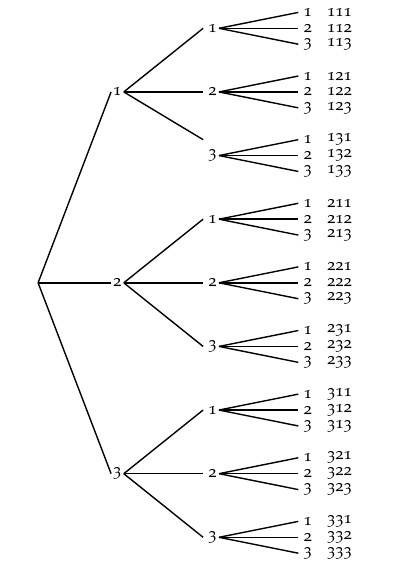
\includegraphics[scale=0.50]{images/arbol_pos.jpg}
\end{center}

%\vskip 8cm
\vskip .2cm ¿Cómo justificamos esto? \pause Por el principio de multiplicación
\end{frame}

\begin{frame}    
    
    De los dos ejemplos anteriores se podría inferir que hay $3^4$ formas posibles de elegir en forma ordenada $4$ elementos del conjunto $1$, $2$, $3$. También, que cuando elijamos $5$ habrá $3^5$ posibilidades y así sucesivamente para enteros más grandes. 

    \pause 

    \vskip .2cm ¿Cómo justificamos esto? \pause     Por el principio de multiplicación

    \pause 

    \vskip .2cm Hemos visto en las página anteriores que hay $3^3$ formas posibles de elegir $3$ números entre $1$, $2$, $3$.

    \vskip .2cm Ahora,  para elegir el cuarto número hay $3$ posibilidades, por lo tanto, por el principio de multiplicación, el número de posibilidades  con cuatro elecciones es
    \begin{equation*}
        3^3 \times 3 = 3^4.
    \end{equation*}
    \end{frame}

\begin{frame}    

    
El razonamiento anterior  se puede extender:

%\begin{proposicion}
\vskip .3cm
{\color{blue} Proposición}
\vskip .2cm
    {\it  Sean  $m,n \in \mathbb N$. Hay   $n^m$ formas posibles de elegir ordenadamente $m$ elementos de un conjunto de $n$ elementos.}
%\end{proposicion}
\vskip .5cm \pause
{\color{blue} Idea de la prueba.} \pause
\vskip .2cm
%\begin{proof}[Idea de la prueba]
    La prueba de esta proposición se basa en aplicar el principio de multiplicación $m-1$ veces, 
    \vskip .2cm
    A nivel formal,  debemos hacer inducción sobre $m$ y usar el principio de multiplicación en el paso inductivo. 

    \qed
%\end{proof}

\end{frame}



\begin{frame}    


%\begin{ejemplo}
    \vskip .3cm
    {\color{blue} Ejemplo}
    \vskip .2cm
    ¿Cuántos números de cuatro dígitos pueden formarse con
    los dígitos $1, 2, 3, 4, 5, 6$?
    \vskip .2cm \pause
    Por la proposición anterior es claro que hay $6^4$ números posibles.
%\end{ejemplo}

%\begin{ejemplo}
\pause
\vskip .8cm
{\color{blue} Ejemplo}
\vskip .2cm
    ¿Cuántos números de $5$ dígitos y capicúas pueden formarse
    con los dígitos $1, 2, 3, 4, 5, 6, 7, 8$? 
    \vskip .2cm \pause
    Un número
    capicúa de cinco dígitos es de la forma
    $$xyzyx$$
    Se reduce a ver cuántos números de tres dígitos pueden
    formarse con aquéllos dígitos. \pause
    Exactamente $8^3$.
%\end{ejemplo}

\end{frame}

\begin{frame}
    
    
        {\color{blue} Ejemplo}
        \vskip .2cm
Sea $X$ un conjunto de $n$ elementos. ¿Cuántos subconjuntos tiene este conjunto?
\vskip .2cm
Por ejemplo, si $X = \{ a, b, c \}$ los subconjuntos de $X$ son:\pause
$$
\emptyset, \{ a \} , \{ b \}, \{ c \}, \{ a, b \}, \{ a, c \}, \{ b, c \}, \{ a, b, c\}.
$$ 
Es decir, si $X$ es un conjunto  de 3 elementos,  entonces tiene $8$ subconjuntos. 
\pause


\vskip .2cm
\begin{tabular}{lll}
    Sea $A \subseteq X$ &$\to$ & $ a \in A$ o  $ a \not\in A$ (2 posibilidades) \\
    &$\to$ & $ b \in A$ o  $ b \not\in A$ (2 posibilidades) \\
    &$\to$ & $ c \in A$ o  $ c \not\in A$ (2 posibilidades) 
\end{tabular}


\vskip .2cm
Luego hay
$$
2 \cdot 2 \cdot 2 = 2^3 = 8
$$
posibles subconjuntos de $X$.  

\end{frame}

\begin{frame}
Razonando de manera análoga obtenemos nuestro primer resultado ``no sencillo'' de conteo. 
\vskip .4cm
%\begin{proposicion} 
{\color{blue}Proposición}
\vskip .2cm
{\it La cantidad de subconjuntos de  un conjunto de $n$ elementos es $2^n$.}
%\end{proposicion}
\vskip .4cm
\pause
Dado  $X$ un conjunto, denotamos $\mathcal P(X)$, \textit{partes de $X$},  al  conjunto  formado por todos los subconjuntos de $X$, por ejemplo
$$
\mathcal P(\{1,2\}) = \{\emptyset,\{1\},\{2\},\{1,2\}\}.
$$  
Si $X$ es un conjunto finito la proposición anterior nos dice que
$$
\mathcal |P(X)| = 2^{|X|}
$$
    
\end{frame}




\begin{frame}    \frametitle{Selecciones ordenadas sin repetición}
    Sea $X$ un conjunto finito de $n$ elementos. 
    
    \vskip .2cm
    \begin{center}
        {\it ¿De cuántas formas podemos elegir $m$  de $X$ en forma ordenada?}
    \end{center}
    \vskip .3cm        \pause 
    %\begin{proposicion} 
    {\color{blue}Ejemplo}
    \vskip .2cm
    Elegir en forma ordenada y sin repetición 2 elementos del conjunto $X = \{ a,b,c\}$,\pause {} tenemos \quad $ ab,\quad ac,\quad ba,\quad bc,\quad ca,\quad cb,$ \quad 
    6  elecciones.
    
    \vskip .5cm    \pause
    
    Es decir si  el conjunto es $X= \{a_1,a_2,\ldots,a_n\}$, las selecciones deben ser del tipo 
    $$
    a_{i_1} a_{i_2} \cdots a_{i_m}
    $$
    donde  $a_{i_j} \not= a_{i_k}$ si $i\not=k$. 
\end{frame}





\begin{frame}        
    Por ejemplo, las selecciones de $3$ elementos en forma ordenada y sin repetición de $\{1, 2,3\}$  son exactamente \pause
    $$
    1 2 3,\; 1 3 2,\; 2 1 3,\; 2 3 1,\; 3 1 2,\; 3 2 1
    $$
    (son las ternas donde los tres números son distintos). 
    
    \vskip .3cm    
    \pause
    O sea hay $6$ selecciones ordenadas y sin repetición de  elementos de $\{1, 2,3\}$.
    \vskip .3cm    
    Notemos que: 
    \vskip .3cm    
    \begin{tabular}{lll}
        $1^{\circ}$ elemento &$\to$ & 3 posibilidades: 1, 2, 3 \\
        $2^{\circ}$ elemento &$\to$ & 2 posibilidades: distinto  al elegido en $1^{\circ}$ \\
        $3^{\circ}$ elemento &$\to$ & 1 posibilidades: distinto  a los elegidos en $1^{\circ}$  y $2^{\circ}$
    \end{tabular}
    \vskip .3cm    
    Tenemos entonces  $3 \cdot 2 \cdot 1 = 3!$ selecciones posibles.
    \vskip .2cm    \vskip .2cm    
\end{frame}


\begin{frame}    
    Pensemos ahora que queremos elegir en forma ordenada y sin repetición $3$ elementos entre $5$. Entonces para la primera elección tenemos $5$ posibilidades, para la segunda $4$ posibilidades y para la tercera $3$ posibilidades haciendo un total de 
    $$
    5 \cdot 4 \cdot 3
    $$
    selecciones posibles. 
    

    \pause
    \vskip .5cm    
    %\begin{proposicion} 
    {\color{blue}Proposición}\label{ordsinrep}
    \vskip .2cm
    {\it Si $n \ge m$ entonces existen
        \begin{equation*}
        n \cdot (n - 1) \cdots (n - m + 1), \qquad \text{($m$ - factores)}
        \end{equation*}
        selecciones ordenadas y sin repetición de $m$ elementos de un conjunto de $n$ elementos.}
    %\end{proposicion}
\end{frame}



\begin{frame}    
    
    
    {\color{blue}Ejemplo}
    \vskip .2cm
    
    Si  hay 10 personas ¿De cuántas formas puedo  hacer una fila de 7 personas?
    \vskip .2cm\pause
    {\color{blue}Solución.}\pause
    \vskip .2cm
    Razonando,
    \vskip .3cm    
    \begin{tabular}{llrl}
        $1^{\circ}$ puesto &$\to$ & 10 &posibilidades \\\pause
        $2^{\circ}$ puesto &$\to$ & 9 &posibilidades\\\pause
        $3^{\circ}$ puesto &$\to$ & 8 &posibilidades \\\pause
        $4^{\circ}$ puesto &$\to$ & 7 &posibilidades \\\pause
        $5^{\circ}$ puesto &$\to$ & 6 &posibilidades\\\pause
        $6^{\circ}$ puesto &$\to$ & 5 &posibilidades \\\pause
        $7^{\circ}$ puesto &$\to$ & 4 &posibilidades \\\pause
    \end{tabular}
    \vskip .3cm    
    La solución es entonces $10 \cdot 9  \cdot 8\cdot 7\cdot 6\cdot 5\cdot 4$.\qed
    
\end{frame}


\begin{frame}    
    
    
    {\color{blue}Ejemplo (repetido)}
    \vskip .2cm
    
    Si  hay 10 personas ¿De cuántas formas puedo  hacer una fila de 7 personas?
    \vskip .2cm\pause
    {\color{blue}Solución (aplicando la proposición de p. \ref{ordsinrep}).}\pause
    \vskip .2cm
    \begin{tabular}{llr}
        Cantidad  de elementos: &$\to$ & $n = 10$ \\\pause
        Cantidad  de elecciones: &$\to$ & $m = 7$
    \end{tabular}
    \vskip .3cm    \pause
    Por lo tanto, $n-m+1 = 10 - 7 +1  = 4$.
    \vskip .3cm    \pause
    La solución es entonces: $10 \cdot 9  \cdot 8\cdot 7\cdot 6\cdot 5\cdot 4$.
    
    \vskip .5cm     \pause
    
    Observar que
    \begin{align*}
    10 \cdot 9  \cdot 8\cdot 7\cdot 6\cdot 5\cdot 4 &= \frac{10 \cdot 9  \cdot 8\cdot 7\cdot 6\cdot 5\cdot 4\cdot 3\cdot 2\cdot1}{3\cdot 2\cdot1} = \frac{10!}{3!} \\
    &= \frac{10!}{(10 -7)!}.
    \end{align*}\qed
    
\end{frame}


\begin{frame}    

    {\color{blue}Ejemplo}
    \vskip .2cm
    ¿Cómo elegir 4 elementos entre $n$?
    \vskip .2cm\pause
    {\color{blue}Solución.}\pause
    \vskip .2cm
    Razonando,
    \vskip .3cm    
    \begin{tabular}{llrl}
        $1^{\circ}$ puesto &$\to$ & n-1 &posibilidades \\\pause
        $2^{\circ}$ puesto &$\to$ & n-2 &posibilidades\\\pause
        $3^{\circ}$ puesto &$\to$ & n-3 &posibilidades \\\pause
        $4^{\circ}$ puesto &$\to$ & n-4 &posibilidades \\\pause
    \end{tabular}

    La solución es entonces 
    \begin{align*}
        (n-1)  (n-2)  (n-3) (n-4) &= \frac{(n-1) (n-2)  (n-3)(n-4) (n-5)!}{(n-5)!}\\
        &=\frac{n!}{(n-5)!}
    \end{align*}
    \qed

\end{frame}

\begin{frame}
    En general
    \begin{equation*}
    n \cdot (n-1)  \cdots (n - m +1) = \frac{    n \cdot (n-1)\cdots (n - m + 1) \cdot (n-m) \cdots 2 \cdot 1 }{(n-m) \cdots 2 \cdot  1 }.
    \end{equation*}
    \vskip .5cm    \pause
    Es decir 

    \setbeamercolor{postit}{fg=black,bg=example text.fg!75!black!10!bg}
    \hskip 1.8cm \begin{beamercolorbox}[wd=0.65\textwidth,rounded=true,shadow=true]{postit}
        \begin{equation*}
        n \cdot (n-1)  \cdots (n - m +1) =  \frac{n!}{(n-m)!}.
    \end{equation*}
    \end{beamercolorbox}    


    \vskip 1cm    \pause
    Por lo tanto podemos reescribir la proposición en forma mas compacta:

    
\end{frame}



\begin{frame}


    {\color{blue}Proposición}
    \vskip .2cm
    {\it Si $n \ge m$ entonces existen
        \begin{equation*}\label{ordenadas_sin_rep_compacta} 
        \frac{n!}{(n-m)!}
        \end{equation*}
        selecciones ordenadas y sin repetición de $m$ elementos de un conjunto de $n$ elementos.}
    %\end{proposicion}
\end{frame}



\begin{frame}
    
    %\begin{ejemplo}
    {\color{blue}Ejemplo}
    \vskip .2cm
    Si en un colectivo hay $9$ asientos vacíos. 
    
    \vskip .2cm
    
    ¿De cuántas formas se pueden distribuir $3$ pasajeros? 
    
    Lo que se está preguntando es cuantas posibles distribuciones de $3$  asientos existen (no importa quien se sienta  en cada asiento). 
    
    
    \vskip .2cm\pause
    {\color{blue}Solución}\pause
    \vskip .2cm
    Se trata de ver cuantas selecciones ordenadas y sin repetición hay de $3$ asientos entre $9$. 
    \vskip .2cm\pause
    Primero hagámoslo usando el principio de multiplicación:\pause
    \vskip .2cm
    \begin{itemize}
        \item 1° persona: 9 lugares posibles. Total: 9\pause
        \item 2° persona: 8 lugares posibles. Total: $9 \times 8$\pause
        \item 3° persona: 7 lugares posibles. Total: $9\times 8\times 7$.
    \end{itemize}
    
\end{frame}



\begin{frame}        
    Este número es
    $$
    9 \cdot 8 \cdot 7 , \qquad \text{$3$ - factores.}
    $$
    %\end{ejemplo}
    \vskip .2cm
    \pause
    Podríamos haberlo hecho directamente por la proposición de la p. \ref{ordenadas_sin_rep_compacta}: elegir  3 elementos entre 9 son
    \vskip .2cm
    \begin{align*}
    \frac{9!}{(9-3)!} &= \frac{9!}{6!} \\
    &= \frac{ 9  \cdot 8\cdot 7\cdot 6\cdot 5\cdot 4\cdot 3\cdot 2\cdot1}{6\cdot 5\cdot 4\cdot 3\cdot 2\cdot1} \\
    &= 9  \cdot 8\cdot 7
    \end{align*}
    posibilidades.
    \qed
\end{frame}




\begin{frame}\frametitle{Permutaciones}
    

    Hay 
    $$
    \frac{n!}{0!}= n!
    $$
    selecciones ordenadas y sin repetición de  $n$ elementos en un conjunto con $n$ elementos. 
    \vskip .4cm\pause
    
    Las selecciones ordenadas y sin repetición de  $n$ elementos en un conjunto con $n$ elementos se denominan {\em permutaciones} de grado $n$.
        \vskip .4cm\pause
    Hay, pues, $n!$ permutaciones de grado $n$.
    \vskip .4cm


\end{frame}

\begin{frame}\frametitle{Permutaciones}

Respondamos la siguiente pregunta:
\vskip .4cm
¿De cuantas formas puedo ordenar $n$ objetos? \pause
\vskip .4cm
Observemos que, ordenar $n$ objetos es equivalente a seleccionar ordenadamente y sin repetición los  $n$ objetos (de un conjunto con $n$ objetos). 
\vskip .4cm
Por lo tanto,  la respuesta es $n!$. \pause
\vskip .4cm
{\color{blue}Ejemplo.}
\vskip .2cm
Dado el conjunto $\mathbb I_4 = \{1,2,3,4 \}$ ¿cuántas permutaciones de los elementos de $\mathbb I_4 $ hay?
\vskip .2cm\pause
{\color{blue}Solución.}\pause $4!$.\qed
\end{frame}



\begin{frame}
    
    {\color{blue}Ejemplo}
    \vskip .2cm
        ¿Cuántas permutaciones pueden formarse con las letras de
        {\em silvia}?
        \pause
        \vskip .2cm
        {\color{blue}Solución}\pause
        \vskip .2cm
        Afirmamos que se pueden formar  $\displaystyle{\frac{6!}{2!}}$ palabras usando las letras de {\em silvia}.
        
        Si escribo en lugar de {\em silvia},
        $$
        \text{\em s i l v i' a}
        $$
        Es decir si cambio la segunda {\em i } por {\em i'}, todas las letras son distintas, luego hay $6!$ permutaciones, pero
        cada par de permutaciones del tipo
        \begin{align*}
        \cdots \text{\em i } \cdots  \text{\em i' }  \cdots \\
        \cdots \text{\em i' } \cdots  \text{\em i } \cdots
        \end{align*}
        coinciden, por lo tanto tengo que dividir por $2$ el número total de permutaciones: $6! / 2! = 360$.\qed
        
\end{frame}


\begin{frame}        Tomemos la palabra
        $$
        \text{\em ramanathan}
        $$
        el número total de permutaciones es $$\displaystyle{\frac{10!}{ 4!2!}}.$$
        \pause
        En efecto, escribiendo el nombre anterior así 
        $$
        r_1\;a_1\;m_1\;a_2\;n_1\;a_3\;t_1\;h_1\;a_4\;n_2
        $$
        el número total de permutaciones es $10!$ Pero
        permutando las $a_i$ y las $n_i$ sin mover las otras letras obtenemos
        la misma permutación de {\em ramanathan}.
        \vskip .2cm
        Como hay $4!$ permutaciones de las letras $a_1$, $a_2$, $a_3$, $a_4$, y
        $2!$ de $n_1$, $n_2$ el número buscado es 
        $$
        \frac{10!}{ 4!2!}.
        $$
        

\end{frame}


\end{document}

